%% -*- coding: utf-8 -*-
\documentclass[12pt,a4paper]{scrartcl} 
\usepackage[utf8]{inputenc}
\usepackage[english,russian]{babel}
\usepackage{indentfirst}
\usepackage{misccorr}
\usepackage{graphicx}
\usepackage{amsmath}
\begin{document}
\section{Введение}
\label{sec:intro}

\subsection{Формулировка задачи}
Программная реализация решения системы линейных алгебраических уравнений методом Гаусса.
\subsection{Краткое описание метода}
Метод Гаусса — классический метод решения системы линейных алгебраических уравнений (СЛАУ). Это метод последовательного исключения переменных, когда с помощью элементарных преобразований система уравнений приводится к равносильной системе треугольного вида, из которой последовательно, начиная с последних (по номеру), находятся все переменные системы.
\subsection{Формулы}
\label{sec:mathexample}

Система линейных уравнений:
\begin{align*}
a_{11}x_1 + a_{12}x_2 + \ldots + a_{1n}x_n &= y_1 \\
a_{21}x_1 + a_{22}x_2 + \ldots + a_{2n}x_n &= y_2 \\
\ldots \\
a_{n1}x_1 + a_{n2}x_2 + \ldots + a_{nn}x_n &= y_n \\
\end{align*}
нормализация уравнений:
\begin{align*}
a_{ij} = \frac{a_{ij}}{a_{ik}}, \quad y_i = \frac{y_i}{a_{ik}}, \quad \text{для } i = k, \quad \text{где } a_{ik} \neq 0
\end{align*}
вычитание уравнений:
\begin{align*}
a_{ij} = a_{ij} - a_{kj}, \quad y_i = y_i - y_k, \quad \text{для } i \neq k
\end{align*}
обратная подстановка:
\begin{align*}
x_k = y_k, \quad x_i = y_i - a_{ik}x_k, \quad \text{для } k = n, n-1, \ldots, 1
\end{align*}

\label{sec:picexample}

\section{Ход работы}
\label{sec:exp}

\subsection{Код приложения}
\label{sec:exp:code}
\begin{verbatim}
#include <iostream>
using namespace std;

// Вывод системы линейных уравнений
void sysout(double** a, double* y, int n)
{
    cout << "Система уравнений:" << endl;
    for (int i = 0; i < n; i++)
    {
        for (int j = 0; j < n; j++)
        {
            cout << a[i][j] << "*x" << j;
            if (j < n - 1)
                cout << " + ";
        }
        cout << " = " << y[i] << endl;
    }
    cout << endl;
}

double* gauss(double** a, double* y, int n)
{
    double* x, max;
    int k, index;
    const double eps = 0.00001; // Точность
    x = new double[n];
    k = 0;

    while (k < n)
    {
        // Поиск строки с максимальным значением a[i][k]
        max = abs(a[k][k]);
        index = k;
        for (int i = k + 1; i < n; i++)
        {
            if (abs(a[i][k]) > max)
            {
                max = abs(a[i][k]);
                index = i;
            }
        }

        // Перестановка строк
        if (max < eps)
        {
            // Проверка отсутствия нулевых диагональных элементов 
            cout << "Решение невозможно из-за нулевого столбца ";
            cout << index << " матрицы A" << endl;
            delete[] x;
            return nullptr;
        }

        for (int j = 0; j < n; j++)
        {
            double temp = a[k][j];
            a[k][j] = a[index][j];
            a[index][j] = temp;
        }

        double temp = y[k];
        y[k] = y[index];
        y[index] = temp;

        // Нормализация уравнений
        for (int i = k; i < n; i++)
        {
            double temp = a[i][k];
            if (abs(temp) < eps)
                continue; // Пропутить для нулевого коэффициента

            for (int j = 0; j < n; j++)
                a[i][j] = a[i][j] / temp;

            y[i] = y[i] / temp;

            if (i == k)
                continue; // Не вычитать уравнение само из себя

            for (int j = 0; j < n; j++)
                a[i][j] = a[i][j] - a[k][j];

            y[i] = y[i] - y[k];
        }

        k++;
    }

    // Обратная подстановка
    for (k = n - 1; k >= 0; k--)
    {
        x[k] = y[k];
        for (int i = 0; i < k; i++)
            y[i] = y[i] - a[i][k] * x[k];
    }

    return x;
}

int main()
{
    setlocale(LC_ALL, "Russian");
    double** a, * y, * x;
    int n;

    cout << "Введите количество уравнений: ";
    cin >> n;

    // Проверка правильности ввода
    while (n <= 0)
    {
        cout << "Число уравнений должно быть целым положительным числом." << endl;
        cout << "Пожалуйста, попробуйте еще раз:";
        cin >> n;
    }

    a = new double* [n];
    y = new double[n];

    // Ввод матрицы A
    cout << endl << "Введите коэффициенты матрицы A:" << endl;
    for (int i = 0; i < n; i++)
    {
        a[i] = new double[n];
        for (int j = 0; j < n; j++)
        {
            cout << "a[" << i << "][" << j << "]= ";
            cin >> a[i][j];
        }
    }

    // Ввод вектора y
    cout << endl << "Введите значения вектора y:" << endl;
    for (int i = 0; i < n; i++)
    {
        cout << "y[" << i << "]= ";
        cin >> y[i];
    }

    cout << endl;

    sysout(a, y, n);

    x = gauss(a, y, n);

    if (x != nullptr)
    {
        cout << "Решение:" << endl;
        for (int i = 0; i < n; i++)
            cout << "x[" << i << "]=" << x[i] << endl;
        delete[] x;
    }

    for (int i = 0; i < n; i++)
        delete[] a[i];
    delete[] a;
    delete[] y;

    cin.ignore();
    cin.get();
    return 0;
}
\end{verbatim}

\section{Работа программы}

Программа начинается с включения необходимых заголовочных файлов и определения некоторых функций.
Далее:
\begin{enumerate}
    \item Функция sysout отвечает за вывод системы линейных уравнений. В качестве входных данных она принимает матрицу a, вектор y и размер системы n. Она выполняет итерации по каждому уравнению и выводит его в виде a[i][j]*x[j] + ... = y[i].

    \item Функция gauss выполняет гауссово исключение для решения системы уравнений. В качестве входных данных она принимает матрицу a, вектор y и размер системы n. Она возвращает массив x, содержащий решения системы уравнений.

    \item Внутри функции gauss объявляется несколько переменных:

- x - динамический массив, используемый для хранения решений системы уравнений.
- max - переменная, используемая для хранения максимального значения, встречающегося в столбце при перестановке строк.
- index - целочисленная переменная, используемая для хранения индекса строки с максимальным значением.
- k - целочисленная переменная, используемая в качестве счетчика цикла.
- eps - постоянная двойная переменная, представляющая порог точности.

    \item Функция начинается с инициализации k в 0, что указывает на первый ряд системы.

    \item Функция входит в цикл, который продолжается до тех пор, пока k не достигнет последней строки системы. В этом цикле выполняются следующие действия:

5.1 Находит строку с максимальным абсолютным значением для текущего столбца a[k][k]. Это называется частичным поворотом. 
5.2 Максимальное значение сохраняется в max, а соответствующий индекс строки - в index.

5.3 Если максимальное значение max ниже порога точности eps, это означает, что решение невозможно из-за нулевого столбца. 
5.4 Функция выводит сообщение об ошибке, освобождает память, выделенную под x, и возвращает nullptr, указывая на невозможность решения.

5.5 Если максимальное значение не ниже порога точности, функция переходит к перестановке строк. Она меняет местами текущую строку a[k] и строку с максимальным значением a[index] в матрице a. Она также меняет местами соответствующие элементы в векторе y.

5.6 Затем функция переходит к нормализации уравнений. Она делит каждый элемент текущей строки на поворотный элемент a[k][k], чтобы поворотный элемент стал равен 1. Она также обновляет соответствующие элементы в векторе y.
Далее функция выполняет операции над строками, чтобы удалить переменные, расположенные ниже поворотного элемента. Она вычитает кратные значения текущей строки a[k] из других строк, делая элементы ниже стержня равными 0.

5.7 Цикл выполняет итерацию, увеличивая k на 1 для перехода к следующей строке, и повторяет описанные выше шаги до тех пор, пока все уравнения не будут нормализованы, а переменные ниже опорных точек не будут устранены.

5.8 После цикла функция переходит в фазу обратной подстановки. Она начинает с последнего уравнения и выполняет обратную подстановку уже найденных значений переменных для решения оставшихся переменных. Она вычисляет значение каждой переменной x[k] путем вычитания из y[k] суммы a[i][k] * x[k] для i от k+1 до n-1.

    \item Функция возвращает массив x, содержащий решения системы уравнений.

    \item С главной функции начинается выполнение программы. Она выполняет следующие действия:

7.1 Объявляются переменные: a (динамический двумерный массив для хранения матрицы a), y (динамический массив для хранения вектора y), x (массив для хранения решений) и n (целочисленная переменная для хранения количества уравнений).

7.2 Программа предлагает пользователю ввести количество уравнений (n) и считывает введенные данные.

7.3 Программа проверяет правильность ввода, убеждаясь, что n - целое положительное число. Если нет, то выводится сообщение об ошибке и пользователю предлагается ввести правильное значение.

7.4 Динамически выделяется память для матрицы a и вектора y в зависимости от размера n.

7.5 Он предлагает пользователю ввести коэффициенты матрицы a и значения вектора y с помощью вложенных циклов.

7.6 Вызывает функцию sysout для вывода на экран системы уравнений, введенной пользователем.
Вызывает функцию gauss для решения системы уравнений и получения решений.

7.7 Если решения существуют (x не является nullptr), то выводит решения на консоль.

7.8 Освобождает память, выделенную для массивов a, x и y.

7.9 Перед выходом программа ждет, пока пользователь нажмет Enter.
\end{enumerate}

Пример работы программы представлен на рис.~\ref{fig:par}.

\begin{figure}[h]
	\centering
	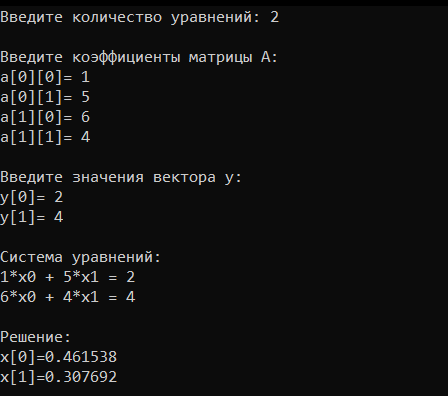
\includegraphics[width=0.8\textwidth]{output.png}
	\caption{Работа программы}\label{fig:par}
 
\end{figure}
\end{document}

